\documentclass{standalone}
\usepackage{tikz}
\usetikzlibrary{patterns, positioning}


\begin{document}
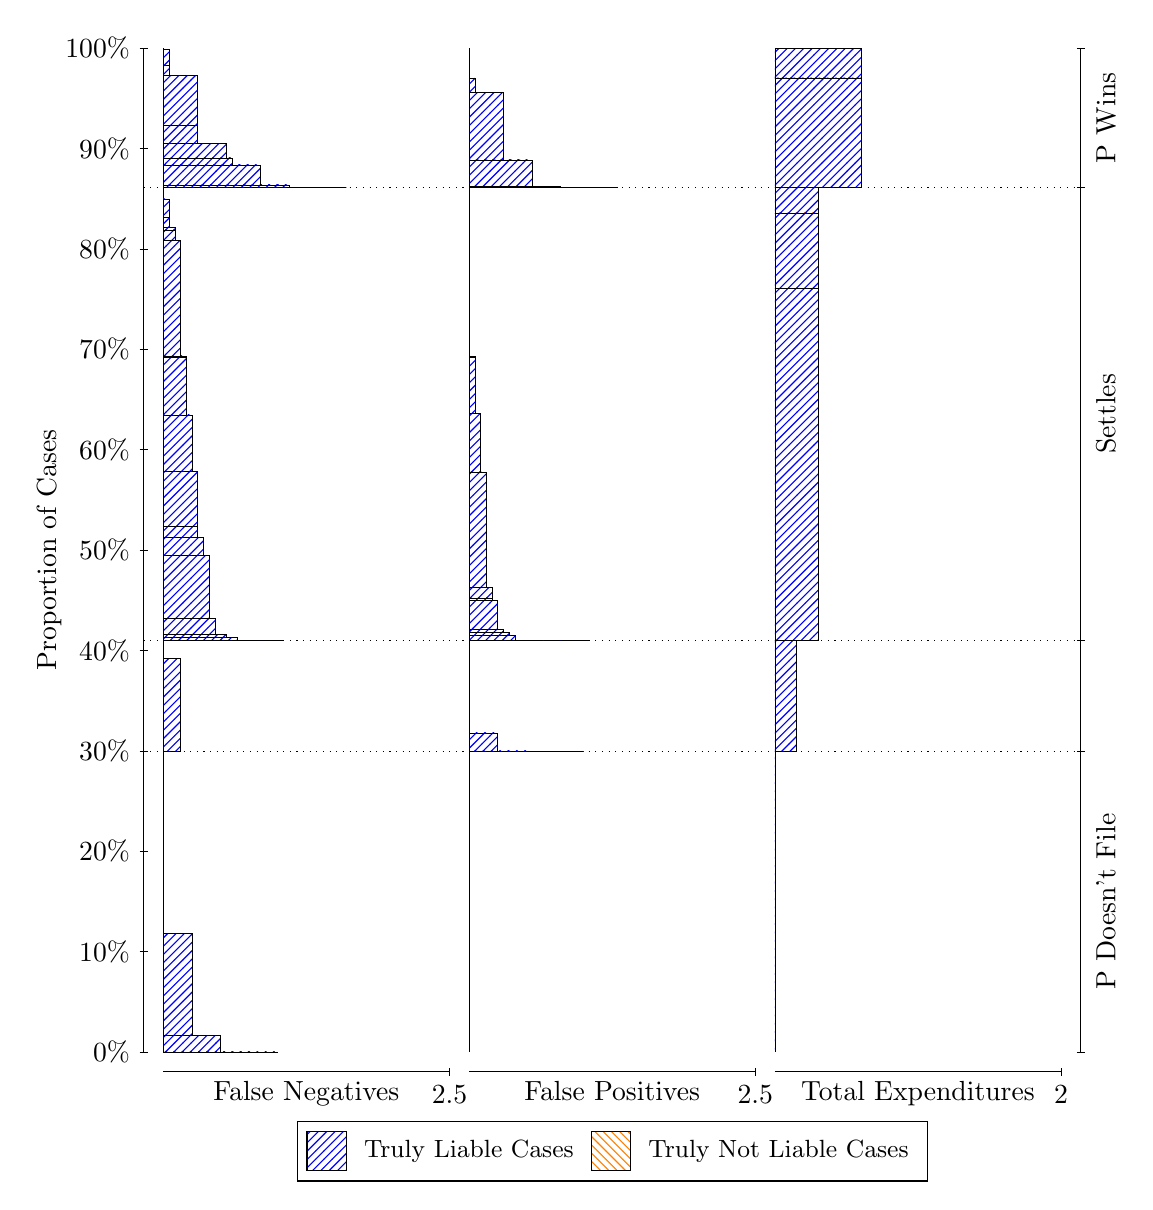
\begin{tikzpicture}
\draw[black, very thin] (1.5,1.75) -- (1.5,14.5);
\node[rotate=90, text=black, anchor=center] at (0.3, 8.125) {Proportion of Cases};
\draw[black, very thin] (1.45,1.75) -- (1.55,1.75);
\node[text=black, anchor=east] at (1.45, 1.75) {0\%};
\draw[black, very thin] (1.45,3.025) -- (1.55,3.025);
\node[text=black, anchor=east] at (1.45, 3.025) {10\%};
\draw[black, very thin] (1.45,4.3) -- (1.55,4.3);
\node[text=black, anchor=east] at (1.45, 4.3) {20\%};
\draw[black, very thin] (1.45,5.575) -- (1.55,5.575);
\node[text=black, anchor=east] at (1.45, 5.575) {30\%};
\draw[black, very thin] (1.45,6.85) -- (1.55,6.85);
\node[text=black, anchor=east] at (1.45, 6.85) {40\%};
\draw[black, very thin] (1.45,8.125) -- (1.55,8.125);
\node[text=black, anchor=east] at (1.45, 8.125) {50\%};
\draw[black, very thin] (1.45,9.4) -- (1.55,9.4);
\node[text=black, anchor=east] at (1.45, 9.4) {60\%};
\draw[black, very thin] (1.45,10.675) -- (1.55,10.675);
\node[text=black, anchor=east] at (1.45, 10.675) {70\%};
\draw[black, very thin] (1.45,11.95) -- (1.55,11.95);
\node[text=black, anchor=east] at (1.45, 11.95) {80\%};
\draw[black, very thin] (1.45,13.225) -- (1.55,13.225);
\node[text=black, anchor=east] at (1.45, 13.225) {90\%};
\draw[black, very thin] (1.45,14.5) -- (1.55,14.5);
\node[text=black, anchor=east] at (1.45, 14.5) {100\%};

\draw[black, very thin] (13.4,1.75) -- (13.4,14.5);
\draw[black, very thin] (13.35,1.75) -- (13.45,1.75);
\node[anchor=west] at (13.35, 1.75) {};
\draw[black, very thin] (13.35,5.5706) -- (13.45,5.5706);
\node[anchor=west] at (13.35, 5.5706) {};
\draw[black, very thin] (13.35,6.9808) -- (13.45,6.9808);
\node[anchor=west] at (13.35, 6.9808) {};
\draw[black, very thin] (13.35,12.726) -- (13.45,12.726);
\node[anchor=west] at (13.35, 12.726) {};
\draw[black, very thin] (13.35,14.5) -- (13.45,14.5);
\node[anchor=west] at (13.35, 14.5) {};

\draw[black, very thin, pattern color=blue, pattern=north east lines] (1.75,1.75) rectangle (3.2033,1.75);
\draw[black, very thin, pattern color=blue, pattern=north east lines] (1.75,1.75) rectangle (2.84,1.7518);
\draw[black, very thin, pattern color=blue, pattern=north east lines] (1.75,1.7518) rectangle (2.4767,1.961);
\draw[black, very thin, pattern color=blue, pattern=north east lines] (1.75,1.961) rectangle (2.1133,3.2569);
\draw[black, very thin, pattern color=orange, pattern=north west lines] (1.75,3.2569) rectangle (1.75,3.2569);
\draw[black, very thin, pattern color=blue, pattern=north east lines] (1.75,3.2569) rectangle (1.75,5.5706);
\draw[black, very thin, pattern color=blue, pattern=north east lines] (1.75,5.5706) rectangle (1.968,6.7502);
\draw[black, very thin, pattern color=orange, pattern=north west lines] (1.75,6.7502) rectangle (1.75,6.7502);
\draw[black, very thin, pattern color=blue, pattern=north east lines] (1.75,6.7502) rectangle (1.75,6.9808);
\draw[black, very thin, pattern color=blue, pattern=north east lines] (1.75,6.9808) rectangle (3.276,6.9808);
\draw[black, very thin, pattern color=blue, pattern=north east lines] (1.75,6.9808) rectangle (3.1307,6.9808);
\draw[black, very thin, pattern color=blue, pattern=north east lines] (1.75,6.9808) rectangle (2.9853,6.9808);
\draw[black, very thin, pattern color=blue, pattern=north east lines] (1.75,6.9808) rectangle (2.9127,6.9808);
\draw[black, very thin, pattern color=blue, pattern=north east lines] (1.75,6.9808) rectangle (2.84,6.9808);
\draw[black, very thin, pattern color=blue, pattern=north east lines] (1.75,6.9808) rectangle (2.7673,6.9808);
\draw[black, very thin, pattern color=blue, pattern=north east lines] (1.75,6.9808) rectangle (2.6947,7.0184);
\draw[black, very thin, pattern color=blue, pattern=north east lines] (1.75,7.0184) rectangle (2.622,7.0193);
\draw[black, very thin, pattern color=blue, pattern=north east lines] (1.75,7.0193) rectangle (2.5493,7.0498);
\draw[black, very thin, pattern color=blue, pattern=north east lines] (1.75,7.0498) rectangle (2.4767,7.0504);
\draw[black, very thin, pattern color=blue, pattern=north east lines] (1.75,7.0504) rectangle (2.404,7.2517);
\draw[black, very thin, pattern color=blue, pattern=north east lines] (1.75,7.2517) rectangle (2.404,7.2525);
\draw[black, very thin, pattern color=blue, pattern=north east lines] (1.75,7.2525) rectangle (2.3313,8.0605);
\draw[black, very thin, pattern color=blue, pattern=north east lines] (1.75,8.0605) rectangle (2.2587,8.2866);
\draw[black, very thin, pattern color=blue, pattern=north east lines] (1.75,8.2866) rectangle (2.186,8.4239);
\draw[black, very thin, pattern color=blue, pattern=north east lines] (1.75,8.4239) rectangle (2.186,9.1226);
\draw[black, very thin, pattern color=blue, pattern=north east lines] (1.75,9.1226) rectangle (2.1133,9.8417);
\draw[black, very thin, pattern color=blue, pattern=north east lines] (1.75,9.8417) rectangle (2.0407,10.575);
\draw[black, very thin, pattern color=blue, pattern=north east lines] (1.75,10.575) rectangle (2.0407,10.59);
\draw[black, very thin, pattern color=blue, pattern=north east lines] (1.75,10.59) rectangle (1.968,12.055);
\draw[black, very thin, pattern color=blue, pattern=north east lines] (1.75,12.055) rectangle (1.8953,12.19);
\draw[black, very thin, pattern color=blue, pattern=north east lines] (1.75,12.19) rectangle (1.8953,12.218);
\draw[black, very thin, pattern color=blue, pattern=north east lines] (1.75,12.218) rectangle (1.8227,12.355);
\draw[black, very thin, pattern color=blue, pattern=north east lines] (1.75,12.355) rectangle (1.8227,12.585);
\draw[black, very thin, pattern color=blue, pattern=north east lines] (1.75,12.585) rectangle (1.75,12.586);
\draw[black, very thin, pattern color=orange, pattern=north west lines] (1.75,12.586) rectangle (1.75,12.586);
\draw[black, very thin, pattern color=blue, pattern=north east lines] (1.75,12.586) rectangle (1.75,12.726);
\draw[black, very thin, pattern color=blue, pattern=north east lines] (1.75,12.726) rectangle (4.0753,12.726);
\draw[black, very thin, pattern color=blue, pattern=north east lines] (1.75,12.726) rectangle (3.712,12.726);
\draw[black, very thin, pattern color=blue, pattern=north east lines] (1.75,12.726) rectangle (3.3487,12.761);
\draw[black, very thin, pattern color=blue, pattern=north east lines] (1.75,12.761) rectangle (3.276,12.761);
\draw[black, very thin, pattern color=blue, pattern=north east lines] (1.75,12.761) rectangle (2.9853,13.015);
\draw[black, very thin, pattern color=blue, pattern=north east lines] (1.75,13.015) rectangle (2.9127,13.015);
\draw[black, very thin, pattern color=blue, pattern=north east lines] (1.75,13.015) rectangle (2.622,13.105);
\draw[black, very thin, pattern color=blue, pattern=north east lines] (1.75,13.105) rectangle (2.5493,13.29);
\draw[black, very thin, pattern color=blue, pattern=north east lines] (1.75,13.29) rectangle (2.2587,13.29);
\draw[black, very thin, pattern color=blue, pattern=north east lines] (1.75,13.29) rectangle (2.186,13.522);
\draw[black, very thin, pattern color=blue, pattern=north east lines] (1.75,13.522) rectangle (2.186,14.148);
\draw[black, very thin, pattern color=blue, pattern=north east lines] (1.75,14.148) rectangle (1.8953,14.148);
\draw[black, very thin, pattern color=blue, pattern=north east lines] (1.75,14.148) rectangle (1.8227,14.282);
\draw[black, very thin, pattern color=blue, pattern=north east lines] (1.75,14.282) rectangle (1.8227,14.481);
\draw[black, very thin, pattern color=orange, pattern=north west lines] (1.75,14.481) rectangle (1.75,14.481);
\draw[black, very thin, pattern color=blue, pattern=north east lines] (1.75,14.481) rectangle (1.75,14.5);
\draw[black, very thin, pattern color=orange, pattern=north west lines] (5.6333,1.75) rectangle (5.6333,1.75);
\draw[black, very thin, pattern color=blue, pattern=north east lines] (5.6333,1.75) rectangle (5.6333,5.5706);
\draw[black, very thin, pattern color=orange, pattern=north west lines] (5.6333,5.5706) rectangle (7.0867,5.5706);
\draw[black, very thin, pattern color=blue, pattern=north east lines] (5.6333,5.5706) rectangle (7.0867,5.5706);
\draw[black, very thin, pattern color=blue, pattern=north east lines] (5.6333,5.5706) rectangle (6.7233,5.5706);
\draw[black, very thin, pattern color=blue, pattern=north east lines] (5.6333,5.5706) rectangle (6.36,5.5724);
\draw[black, very thin, pattern color=blue, pattern=north east lines] (5.6333,5.5724) rectangle (5.9967,5.8012);
\draw[black, very thin, pattern color=blue, pattern=north east lines] (5.6333,5.8012) rectangle (5.6333,6.9808);
\draw[black, very thin, pattern color=orange, pattern=north west lines] (5.6333,6.9808) rectangle (7.1593,6.9808);
\draw[black, very thin, pattern color=blue, pattern=north east lines] (5.6333,6.9808) rectangle (7.1593,6.9808);
\draw[black, very thin, pattern color=orange, pattern=north west lines] (5.6333,6.9808) rectangle (7.014,6.9808);
\draw[black, very thin, pattern color=blue, pattern=north east lines] (5.6333,6.9808) rectangle (7.014,6.9808);
\draw[black, very thin, pattern color=orange, pattern=north west lines] (5.6333,6.9808) rectangle (6.8687,6.9808);
\draw[black, very thin, pattern color=blue, pattern=north east lines] (5.6333,6.9808) rectangle (6.8687,6.9808);
\draw[black, very thin, pattern color=blue, pattern=north east lines] (5.6333,6.9808) rectangle (6.796,6.9808);
\draw[black, very thin, pattern color=orange, pattern=north west lines] (5.6333,6.9808) rectangle (6.7233,6.9808);
\draw[black, very thin, pattern color=blue, pattern=north east lines] (5.6333,6.9808) rectangle (6.7233,6.9808);
\draw[black, very thin, pattern color=blue, pattern=north east lines] (5.6333,6.9808) rectangle (6.6507,6.9808);
\draw[black, very thin, pattern color=orange, pattern=north west lines] (5.6333,6.9808) rectangle (6.578,6.9808);
\draw[black, very thin, pattern color=blue, pattern=north east lines] (5.6333,6.9808) rectangle (6.578,6.9808);
\draw[black, very thin, pattern color=blue, pattern=north east lines] (5.6333,6.9808) rectangle (6.5053,6.9808);
\draw[black, very thin, pattern color=blue, pattern=north east lines] (5.6333,6.9808) rectangle (6.4327,6.9809);
\draw[black, very thin, pattern color=orange, pattern=north west lines] (5.6333,6.9809) rectangle (6.4327,6.9809);
\draw[black, very thin, pattern color=blue, pattern=north east lines] (5.6333,6.9809) rectangle (6.4327,6.9809);
\draw[black, very thin, pattern color=blue, pattern=north east lines] (5.6333,6.9809) rectangle (6.36,6.9811);
\draw[black, very thin, pattern color=blue, pattern=north east lines] (5.6333,6.9811) rectangle (6.2873,6.9812);
\draw[black, very thin, pattern color=orange, pattern=north west lines] (5.6333,6.9812) rectangle (6.2873,6.9812);
\draw[black, very thin, pattern color=blue, pattern=north east lines] (5.6333,6.9812) rectangle (6.2873,6.9815);
\draw[black, very thin, pattern color=blue, pattern=north east lines] (5.6333,6.9815) rectangle (6.2147,7.0453);
\draw[black, very thin, pattern color=orange, pattern=north west lines] (5.6333,7.0453) rectangle (6.142,7.0453);
\draw[black, very thin, pattern color=blue, pattern=north east lines] (5.6333,7.0453) rectangle (6.142,7.0793);
\draw[black, very thin, pattern color=blue, pattern=north east lines] (5.6333,7.0793) rectangle (6.0693,7.1207);
\draw[black, very thin, pattern color=blue, pattern=north east lines] (5.6333,7.1207) rectangle (6.0693,7.1212);
\draw[black, very thin, pattern color=orange, pattern=north west lines] (5.6333,7.1212) rectangle (5.9967,7.1212);
\draw[black, very thin, pattern color=blue, pattern=north east lines] (5.6333,7.1212) rectangle (5.9967,7.4888);
\draw[black, very thin, pattern color=blue, pattern=north east lines] (5.6333,7.4888) rectangle (5.924,7.5167);
\draw[black, very thin, pattern color=blue, pattern=north east lines] (5.6333,7.5167) rectangle (5.924,7.651);
\draw[black, very thin, pattern color=blue, pattern=north east lines] (5.6333,7.651) rectangle (5.8513,9.1161);
\draw[black, very thin, pattern color=blue, pattern=north east lines] (5.6333,9.1161) rectangle (5.7787,9.8648);
\draw[black, very thin, pattern color=blue, pattern=north east lines] (5.6333,9.8648) rectangle (5.706,10.569);
\draw[black, very thin, pattern color=blue, pattern=north east lines] (5.6333,10.569) rectangle (5.706,10.584);
\draw[black, very thin, pattern color=blue, pattern=north east lines] (5.6333,10.584) rectangle (5.6333,12.726);
\draw[black, very thin, pattern color=orange, pattern=north west lines] (5.6333,12.726) rectangle (7.5227,12.726);
\draw[black, very thin, pattern color=blue, pattern=north east lines] (5.6333,12.726) rectangle (7.5227,12.726);
\draw[black, very thin, pattern color=orange, pattern=north west lines] (5.6333,12.726) rectangle (7.1593,12.726);
\draw[black, very thin, pattern color=blue, pattern=north east lines] (5.6333,12.726) rectangle (7.1593,12.726);
\draw[black, very thin, pattern color=orange, pattern=north west lines] (5.6333,12.726) rectangle (6.796,12.726);
\draw[black, very thin, pattern color=blue, pattern=north east lines] (5.6333,12.726) rectangle (6.796,12.745);
\draw[black, very thin, pattern color=orange, pattern=north west lines] (5.6333,12.745) rectangle (6.4327,12.745);
\draw[black, very thin, pattern color=blue, pattern=north east lines] (5.6333,12.745) rectangle (6.4327,13.078);
\draw[black, very thin, pattern color=orange, pattern=north west lines] (5.6333,13.078) rectangle (6.36,13.078);
\draw[black, very thin, pattern color=blue, pattern=north east lines] (5.6333,13.078) rectangle (6.36,13.078);
\draw[black, very thin, pattern color=blue, pattern=north east lines] (5.6333,13.078) rectangle (6.0693,13.936);
\draw[black, very thin, pattern color=orange, pattern=north west lines] (5.6333,13.936) rectangle (5.9967,13.936);
\draw[black, very thin, pattern color=blue, pattern=north east lines] (5.6333,13.936) rectangle (5.9967,13.936);
\draw[black, very thin, pattern color=blue, pattern=north east lines] (5.6333,13.936) rectangle (5.706,14.12);
\draw[black, very thin, pattern color=orange, pattern=north west lines] (5.6333,14.12) rectangle (5.6333,14.12);
\draw[black, very thin, pattern color=blue, pattern=north east lines] (5.6333,14.12) rectangle (5.6333,14.5);
\draw[black, very thin, pattern color=orange, pattern=north west lines] (9.5167,1.75) rectangle (9.5167,1.75);
\draw[black, very thin, pattern color=blue, pattern=north east lines] (9.5167,1.75) rectangle (9.5167,5.5706);
\draw[black, very thin, pattern color=orange, pattern=north west lines] (9.5167,5.5706) rectangle (9.7892,5.5706);
\draw[black, very thin, pattern color=blue, pattern=north east lines] (9.5167,5.5706) rectangle (9.7892,6.9808);
\draw[black, very thin, pattern color=orange, pattern=north west lines] (9.5167,6.9808) rectangle (10.062,6.9808);
\draw[black, very thin, pattern color=blue, pattern=north east lines] (9.5167,6.9808) rectangle (10.062,11.448);
\draw[black, very thin, pattern color=orange, pattern=north west lines] (9.5167,11.448) rectangle (10.062,11.448);
\draw[black, very thin, pattern color=blue, pattern=north east lines] (9.5167,11.448) rectangle (10.062,12.407);
\draw[black, very thin, pattern color=orange, pattern=north west lines] (9.5167,12.407) rectangle (10.062,12.407);
\draw[black, very thin, pattern color=blue, pattern=north east lines] (9.5167,12.407) rectangle (10.062,12.726);
\draw[black, very thin, pattern color=orange, pattern=north west lines] (9.5167,12.726) rectangle (10.607,12.726);
\draw[black, very thin, pattern color=blue, pattern=north east lines] (9.5167,12.726) rectangle (10.607,14.12);
\draw[black, very thin, pattern color=orange, pattern=north west lines] (9.5167,14.12) rectangle (10.607,14.12);
\draw[black, very thin, pattern color=blue, pattern=north east lines] (9.5167,14.12) rectangle (10.607,14.5);
\draw[black, dotted] (1.5,5.5706) -- (13.4,5.5706);
\draw[black, dotted] (1.5,6.9808) -- (13.4,6.9808);
\draw[black, dotted] (1.5,12.726) -- (13.4,12.726);
\draw[black, very thin] (1.75,1.5) -- (5.3833,1.5);
\node[text=black, anchor=north] at (3.5667, 1.5) {False Negatives};
\draw[black, very thin] (5.3833,1.45) -- (5.3833,1.55);
\node[text=black, anchor=north] at (5.3833, 1.45) {2.5};

\draw[black, very thin] (5.6333,1.5) -- (9.2667,1.5);
\node[text=black, anchor=north] at (7.45, 1.5) {False Positives};
\draw[black, very thin] (9.2667,1.45) -- (9.2667,1.55);
\node[text=black, anchor=north] at (9.2667, 1.45) {2.5};

\draw[black, very thin] (9.5167,1.5) -- (13.15,1.5);
\node[text=black, anchor=north] at (11.333, 1.5) {Total Expenditures};
\draw[black, very thin] (13.15,1.45) -- (13.15,1.55);
\node[text=black, anchor=north] at (13.15, 1.45) {2};

\node[text=black, centered, rotate=90] at (13.72, 3.6603) {P Doesn't File};

\node[text=black, centered, rotate=90] at (13.72, 9.8533) {Settles};
\node[text=black, centered, rotate=90] at (13.72, 13.613) {P Wins};

\draw (7.449999999999999,1.5) node[draw=none] (baseCoordinate) {};
\begin{scope}[align=center]
        \matrix[scale=0.5, draw=black, below=0.5cm of baseCoordinate, nodes={draw}, column sep=0.1cm]{
            \node[rectangle, draw, minimum width=0.5cm, minimum height=0.5cm, pattern color=blue, pattern=north east lines] {}; &
            \node[draw=none, font=\small, text=black] (B) {Truly Liable Cases}; &
            \node[rectangle, draw, minimum width=0.5cm, minimum height=0.5cm, pattern color=orange, pattern=north west lines] {}; &
            \node[draw=none, font=\small, text=black] (B) {Truly Not Liable Cases}; \\
            };
\end{scope}

\end{tikzpicture}
\end{document}